\section{Approach} \label{approach}
In this Chapter, we describe how we went about the creation of our data structure and what the different considerations were. This includes the high-level ideas that resulted in our data structure. We also include a section explaining the required steps for running simulations inside the VDB data structure, unfortunately, this was not implemented. We then continue with the animation setup and the compression scheme used for our voxel data.




\subsection{VDB data structure} \label{approach:vdb_data_structure}
The data structure of choice is VDB. This is a compromise between ray tracing performance and compression, and can be extended or reshaped (internal layers could be removed, added or changed in size) if desired. However, the top-level node, which can be indefinitely large, was not used. This removes the need to perform the expansive hash table step and also removes the need for our accessor types. Additionally, this restricts our index space to a certain region. In our implementation, we chose the standard 5-4-3 VDB layout resulting in an index space of $1 << (5+4+3) = 4096$ cubed. More than large enough for most VDB files. This has a few implications: an empty volume uses $((1<<5)^3+((1<<5+4)^3)) / 8 = 16$MB because we always allocate 1 top-level node along with one 2nd level node for every bit in the top level node's bit mask. There are also always 3 indirections before we can access our voxel data. Our large higher-level nodes will rarely contain duplicates (as required by SVDAG, described in Section \ref{related_work:voxel_data_structures:svdag}).

\subsection{Simulation} \label{approach:simulation}
As part of implementing a dynamic VDB data structure, there was some work done regarding a GPU-modifiable version. Unfortunately, due to time constraints, this was never fully implemented or tested. However, there were some findings about how such a system could be implemented.

Modifying a sparse volume data structure on the GPU has many inherent issues. One of those issues arises because the GPU is a massively parallel system that requires cautious handling of synchronization. When implementing a VDB-like structure with 3 indirections (top-level node, 2 internal layers, and the voxel data) we have to make sure that all parent nodes are present. One way of doing this would be to check if the parent exists, if not, we create it. We can create the parent node by keeping track of an atomic counter which is used for indexing into a large buffer in which we allocate our parent. However, what if we allocate two voxels with the same parent, then we will allocate twice and have the parents parent point to one of the allocated nodes. This is a race condition.

Let's say we tried to use that scheme, but we use one of the essential parts of the VDB data structure, the bit mask. So we use an atomic bitwise or operation on the bit mask which sets the correct bit to true. This operation will also return the original output, which for one thread will be false, and for all other threads that did the atomic operation, will be true. So now we have a single thread that can allocate the node and set the parent's parent pointer right? Well no, the GPU can, at any time, swap out the currently running warp. So one warp can set the bit, and be responsible for setting the parent's parent pointer, but it is being swapped out. This would result in other threads assuming that the pointer is already set, and them accessing garbage data.

So the only real way to handle this situation is to set the bits and pointers without reading either of these values within the same dispatch. This necessitates the separation of the initialization of the different layers of the tree into different dispatches. However, this does raise a new problem, how do we know which top-level nodes to allocate and which bits to set? We could iterate over our entire dataset for every dispatch to find which nodes have to be allocated, but this might be wasteful if our dataset is large.

To conclude, if an editable VDB data structure is desired, it can be done. However, it will necessitate the use of at least 3 dispatches which might all need to access the entire dataset (as show in Figure \ref{fig:VDB_simulation_construction}). If the dataset is not too big this might be fine because of the GPU's high bandwidth.

\begin{figure}[H]
    \centering
    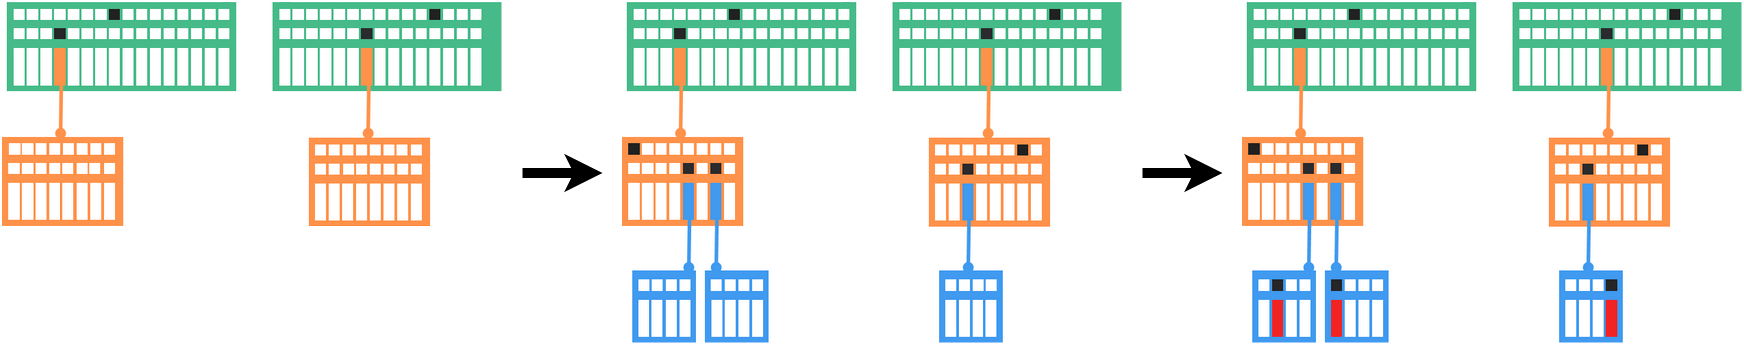
\includegraphics[width=0.9\linewidth]{figures/VDB construction.png}
    \caption{Construction of the VDB data structure in 3 steps. These steps are separated by arrows which indicate the different dispatches with barriers between them. This ensures that all work in the upper level of the tree has been done before continuing to the lower levels. The first step is to build set our top level bit masks and pointers. Then, in the next dispatch, we set our internal node bit masks and pointers. And lastly we set our lowest level node pointers and bit masks. After this dispatch we can start placing our voxel values. }
    \label{fig:VDB_simulation_construction}
\end{figure}

\subsection{Flip book animations} \label{approach:flipbook_animations}
Flip book animations are the opposite of delta compression. It means that we store every frame as a separate data structure, disregarding any temporal coherency. So why mention them, when they are not what we need? If we look at the actual data being used we see that by far the largest amount of memory is being used by the actual voxel data. Depending on what tree structure we use, this can be a larger or smaller part of our structure. This leads to another interesting observation. If all these data structures use voxels as their leaf values, they could all share these leaf values. We can build different structures on top of a set of voxel bricks. For example, we can have a set of bricks in a brick map to run a simulation, then mesh these bricks, so we can use the hardware rasterizer to find primary intersections. After which we can traverse them using DDA (see Section \ref{related_work:attribute_separation:fast_volume_traversal}) and do our shading. All these operations utilize the same underlying voxel data. So if we can get that as small as possible, we should be able to use an appropriate 'interface' to our data and have exactly what we need. Whether this is a flat or deep tree or even something like a triangle mesh or BVH. This is why we mostly look at compressing our voxel brick data as much as possible. For animations, we have thus decided to use a simple flip book animation for the tree, while using one large voxel brick buffer.

\subsection{Texture compression} \label{approach:texture_compression}
Keeping our voxel brick data in a large buffer can only do so much on the GPU. We are bound by 32-bit loads, have to set up a cache-friendly access structure ourselves, and most importantly, cannot use block compression (this only works on textures as it uses spatial coherence to compress). This is why the voxel data is stored in a sampled 3D texture. Using this texture we automatically get optimized access to our voxel data in the same way that 2D textures have fast access for filtering. The actual bricks should now be stored in texture slices. So, we can create a texture with a certain width, height and depth (divisible by 8, our brick size), then move each of our voxels from the old brick buffer to our new brick texture.


To compress our data there are a few new possibilities. Because we can skip these 32-bit loads, we can easily store 16-bit floating point or unsigned normalized values (8-bit floating point values between 0 and 1). These normalized values can be denormalized to get the original values back. So now we have an easy way of reducing our voxel data by $4\times$. But we can go even further. BC4 (See Section \ref{related_work:texture_compression}) is a block compression method made for grayscale values, perfect for our density values. It encodes grayscale values at $0.5$ byte/pixel, meaning that we can store two voxels per byte. This already shrinks our data from 32bit per voxel to 4bits, an eight times reduction. However, we can use one last optimization using block compression. If we recall how block compression works, we see that it somehow compresses $4\times 4$ pixels. Now if we use one of the block compression techniques which encodes full RGBA data we get four floating point numbers per pixel, resulting in $4 \times 4 \times 4$ values. We can exploit this by storing our voxel data as separate color channels in our texture. When using either BC7 or BC3 we can encode floating point values at 1 byte/pixel. However, each of our pixels contains four density values, thus shrinking our volume data even further to a rate of 2bits per voxel. This is a sixteen-times reduction over using full 32-bit floating point values. A slice of the resulting texture can be seen in Figure \ref{fig:vdb_asset:memory_view}.

\subsection{Clustering similar nodes} \label{approach:clustering_similar_nodes}
The fundamental idea behind compression is the reduction of duplicates. But when using volume data, or any floating point data, there is a low chance of having exact duplicate data. When looking at large-volume datasets however, there is a decent chance that two bricks will have roughly the same data. This can be the almost homogeneous area inside a cloud or a non-moving part of an animation for example. We can identify these similar bricks using clustering. This idea was inspired by \cite{van2020lossy} where they performed clustering on the voxel geometry. However, unlike that technique, we specifically want our density data to be compressed. So we perform k-means clustering \cite{macqueen1967some} using the normalized Manhattan distance, between 5 and 15 iterations and $k$ is the desired number of new bricks. However, there are two issues with this which can be worked around. (1) low-density bricks will always be similar, and (2) bricks that are similar for almost all density values except for a few, result in high similarity, yet we lose a lot of important detail. Both of these issues can be negated by introducing a variance threshold. We normalize all density values inside a brick, and then calculate the variance of all values in the brick. If this is above some set threshold we simply do not include it in our clustering, and keep using the original value. This way we do lose the ability to cluster smooth gradients, but we do make sure that we keep as much detail as we want. DBSCAN \cite{ester1996density} was also considered, but it did not seem like a good fit as we specifically only want to cluster bricks that are similar to each other. We do not want DBSCAN to form large chains where two end-points of the cluster are vastly different.